\section{Auswertung}

\subsection{Überprüfung der Bragg-Bedingung}

Bei einem Kristallwinkel von $\theta_{\text{K}} = 14{\textdegree}$ wurde der Winkel $\theta_{\text{GM}}$ vom Geiger-Müllerzählrohr variiert und die Zählrate gemessen.
Die Werte sind in der Tabelle \ref{tab:ogemessdaten1} angegeben und lassen sich nun in ein Diagramm \ref{fig:plot1} mit Winkelabhängigkeit einzeichnen.
\begin{figure}[h]
  \centering
  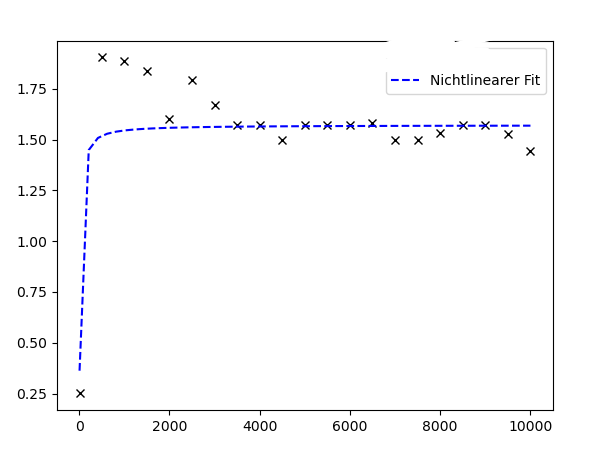
\includegraphics[width=\textwidth]{build/plot1.pdf}
  \caption{Zählratendiagramm mit Winkelabhängigkeit.}
  \label{fig:plot1}
\end{figure}
Der Winkel mit der höchsten Zählrate lässt sich am Diagramm \ref{fig:plot1} und an den Messwerten \ref{tab:ogemessdaten1} als
\begin{equation}
\theta_{\text{max}} = 28{,}2{\textdegree}
\end{equation}
feststellen.
Die theoretische Lage des Maximums ist bei fest eingestellten 14$\textdegree$ des Kristalls genau das doppelte. Also hat der Sollwert einen Winkel von $\theta_{\text{soll}} = 28{\textdegree}$. Es ergibt sich folgende Abweichung vom Sollwert.
\begin{equation}
\increment \theta_{\text{ges}} = \theta_{\text{max}} - \theta_{\text{soll}} = 0{,}2{\textdegree}
\end{equation}
Im folgenden stellt sich also aus geometrischen Gründen ein Fehler auf den Winkel $\theta$ von
\begin{equation}
\label{eqn:fehlerwinkel}
\increment \theta = 0{,}1{\textdegree}
\end{equation}
ein. Dieser bezieht sich also nicht mehr auf den gesamten Winkel sondern nur noch auf den Ausfallenden, der bei Verwendung der Bragg-Bedingung \eqref{eqn:braggEnergy}
verwendet wird.

\subsection{Analyse eines Emissionsspektrums einer Kupfer-Röntgenröhre}

Das Emissionsspektrum wurde mit einer Integrationszeit von $\increment t = \SI{10}{\second}$ in jeweils $\increment \theta = 0{,}1\textdegree$ Abständen gemessen.
Die ermittelten Zählraten sind poissonverteilt, somit lässt sich der Fehler gemäß
\begin{equation}
\increment N_{i} = \sqrt{N_{i}}
\end{equation}
berechnen. Diese Werte lassen sich nun mit einem Fehlerbalken in ein Diagramm \ref{fig:plot2} eintragen wobei die Charakteristik des Zählrohrs gut zu erkennen ist.
Der Bremsberg ist im Diagramm durch schwarze Punkte dargestellt, sie zeigen die Strahlung welche durch Abbremsung der Elektronen am Kupfer entsteht. 
Außerdem sind zwei charakteristische Linien zu erkennen, die $K_{\beta}$ und $K_{\alpha}$-Linie. 
Die Maxima dieser Linien liegen bei.
\begin{align}
K_{\alpha} &= (20{,}2 \pm 0{,}1)\textdegree \\
K_{\beta} &= (22{,}5 \pm 0{,}1)\textdegree
\end{align}
Der Fehler stammt aus der Überprüfung der Bragg-Bedingung \eqref{eqn:fehlerwinkel}.
Sie zeigen jeweils die Winkeleinstellung, bei der ein Photon durch das zurückfallen eines Elektrons auf eine
niedrigere Schale, in dem Fall von $n=2$ auf $n=1$ für $K_{\alpha}$ und von $n=3$ auf $n=1$ für $K_{\beta}$, am Kristall reflektiert wird. 
An den ermittelten Werten lässt sich keine minimale Wellenlänge und keine maximale Energie des Bremsbergs bestimmen. Für Information auf die minimale Wellenlänge müsste bei einer geringe Winkeleinstellung
gemessen werden damit der Punkt sichtbar wird, wo die Zählrate noch auf Null steht. Der Bremsberg verläuft relativ linear in dem gemessenen Winkelbereich und fällt nur schwach ab, daraus lässt sich kein
aussagekräftiges Maximum erkennen. 
\subsubsection{Halbwertsbreite}
Für jede charakteristische Linie kann eine Halbwertsbreite ermittelt werden, dazu wird das Intensitätsmaximum halbiert und die Werte links und rechts neben dem Maximum die diesen Wert
annehmen bestimmen die Halbwertsbreite.
Zunächst hat $K_{\beta}$ eine halbierte Peakintensität von $N_{\beta} = \SI{2525}{{\text{Imp}}\per\second}$ die gemessenen Werte liegen zwischen diesem Wert, deshalb kann eine
lineare Approximation verwendet werden. Es gilt.
\begin{equation}
2525 = \frac{P_{2}-P_{1}}{0{,}1} \cdot \theta + P_{1}
\end{equation}
Dabei ist $P_{2}$ der Punkt der gerade über der halben Peakintensität ist und $P_{1}$ der, welcher gerade darunter liegt.
Dies kann nach $\theta$ umgeformt werden und auf den Wert $\theta_{P_{1}}$ addiert werden. Es ergibt sich also der Punkt der Halbwertsbreite links vom Maximum.
\begin{equation}
\theta_{\text{links}} = 0{,}1 \cdot \frac{2525-P_{1}}{P_{2}-P_{1}} + \theta_{P_{1}}
\end{equation}
Es ergeben sich die Werte.
\begin{align}
\theta_{K_{\beta}\text{,links}} &= (22{,}35 \pm 0{,}1)\textdegree\\
\theta_{K_{\beta}\text{,rechts}} &= (22{,}85\pm 0{,}1)\textdegree
\end{align}
Der Fehler entsteht dabei durch die Fehlerbehaftung von $\theta_{P_{1}}$ von $\increment \theta_{P_{1}} = 0{,}1\textdegree$ aus der Überprüfung der Bragg-Bedingung.
Für die rechte Seite muss dabei beachtet werden, dass sich das Vorzeichen der Steigung ändert.
Die Halbwertsbreite für $K_{\beta}$ ist also.
\begin{equation}
\text{FWHM}_{K_{\beta}} = \theta_{K_{\beta}\text{,rechts}} - \theta_{K_{\beta}\text{,links}} = (0{,}5 \pm 0{,}14)\textdegree
\end{equation}
FWHM steht dabei für \enquote{Full Width at Half Maximum}.
Mit einer analogen Rechnung für $K_{\alpha}$ ergeben sich die folgenden Werte.
\begin{align}
\theta_{K_{\alpha}\text{,links}} &= (20{,}06\pm 0{,}1)\textdegree \\
\theta_{K_{\alpha}\text{,rechts}} &= (20{,}55\pm 0{,}1)\textdegree \\
\text{FWHM}_{K_{\alpha}} &=  (0{,}49 \pm 0{,}14)\textdegree
\end{align}
Die Halbwertsbreiten sind ebenfalls in das Diagramm \ref{fig:plot2} eingezeichnet.
\begin{figure}[h]
  \centering
  \includegraphics[width=\textwidth]{build/plot2.pdf}
  \caption{Röntgenspektrum einer Kupfer-Röntgenröhre.}
  \label{fig:plot2}
\end{figure}
Die Fehler auf den Halbwertsbreiten ergeben sich durch eine Gaußsche Fehlerfortpflanzung.
\begin{equation}
\increment \text{FWHM}_{K_{\text{i}}} = \sqrt{(\increment \theta_{K_{\text{i}}\text{,rechts}})^{2} + (\increment \theta_{K_{\text{i}}\text{,links}})^{2}}
\end{equation}
\subsubsection{Auflösevermögen}
Für das Auflösevermögen müssen die Energien der charakteristischen Linien $E_{K}$ bestimmt werden, sowie die Energiedifferenz der Halbwertsbreiten $\increment E_{\text{FWHM}}$.
Das Auflösevermögen $A$ lässt sich durch
\begin{equation}
\label{eqn:gg}
A = \frac{E_{K}}{\increment E_{\text{FWHM}}}
\end{equation}
errechnen. Dabei lassen sich die Energien nach der Gleichung \eqref{eqn:braggEnergy} bestimmen.
Die folgende Wertetabelle gibt die Ergebnisse an.
\begin{table}
\centering
\caption{Energien der charakteristischen Linien zur Bestimmung des Auflösevermögen.}
\label{tab:lol}
\begin{tabular}{c c c c c}
    \toprule
    Linie & $E_{\text{peak}}$[$\si{\kilo\electronvolt}$] & $E_{\text{FWHM,links}}$[$\si{\kilo\electronvolt}$] & $E_{\text{FWHM,rechts}}$[$\si{\kilo\electronvolt}$] & $\increment E_{\text{FWHM}}$[$\si{\kilo\electronvolt}$] \\
    \midrule
    $K_{\alpha}$ & $\SI{8.043(34)}{}$& $\SI{8.974(43)}{}$& $\SI{8.769(41)}{}$ & $\SI{0.205(59)}{}$\\
    $K_{\beta}$ &$\SI{8.914(42)}{}$ &$\SI{8.095(34)}{}$ &$\SI{7.927(33)}{}$ & $\SI{0.168(48)}{}$ \\
    \bottomrule
\end{tabular}
\end{table}
\\
Die Fehler entspringen der folgenden Fehlerfortpflanzung.
\begin{equation}
\label{eqn:fehleritin}
\increment E_{\text{i}} = \frac{h \cdot c \cdot \text{cos}(\theta_{\text{i}})}{2 \cdot d \cdot {\text{sin}(\theta_{\text{i}})}^{2}} \cdot \increment \theta_{\text{i}}
\end{equation}
Diese Werte lassen sich nun in die Gleichung \eqref{eqn:gg} einsetzen und es folgen zwei Werte des Auflösevermögens für die beiden Linien.
\begin{align}
A_{K_{\alpha}} &= \SI{39.23(1133)}{} \\
A_{K_{\beta}} &= \SI{53.08(1502)}{}
\end{align}
Hier werden die Fehler durch die beiden fehlerbehafteten Energieterme mit folgender Fehlerfortpflanzung bestimmt.
\begin{equation}
\increment A_{\text{i}} = \sqrt{\left( \frac{1}{E_{\text{FWHM}}}\right)^{2} (\increment E_{\text{K}})^{2} + \left( \frac{E_{\text{K}}}{{E_{\text{FWHM}}}^{2}}\right)^{2} (\increment E_{\text{FWHM}})^{2}}
\end{equation}

\subsubsection{Bestimmung der Abschirmkonstanten}
Aus den Gleichungen \eqref{eqn:sommerfeldenergie} und \eqref{eqn:kackeq} lassen sich bei Vernachlässigung des Drehimpulsbeitrages die Abschirmkonstanten für Kupfer folgendermaßen angeben.
\begin{align}
\label{eqn:11}
\sigma_1 &= Z_{\text{Cu}} - \sqrt{\frac{E_{\symup{K,abs}}}{R_{\infty}} } \\
\sigma_2 &= Z_{\text{Cu}} - 2 \sqrt{\frac{R_{\infty}(Z_{\text{Cu}} - \sigma_1)^2 - E_{\symup{K_{\alpha}}}}{R_{\infty}}} \\
\label{eqn:33}
\sigma_3 &= Z_{\text{Cu}} - 2 \sqrt{\frac{R_{\infty}(Z_{\text{Cu}} - \sigma_1)^2 - E_{\symup{K_{\beta}}}}{R_{\infty}}} 
\end{align}
Für die Berechnung von $\sigma_1$ wird die Absorptionsenergie der K-Kante benötigt hierzu wird ein Literaturwert zur Rate gezogen.
Dieser ist nach \cite{random}.
\begin{equation}
E_{\symup{K,abs}} = \SI{8987.96}{\electronvolt}
\end{equation}
Dieser Wert kann nun zusammen mit den bereits bestimmten Energien an den Peaks der $K_{\alpha}$ und $K_{\beta}$-Linie aus Tabelle \ref{tab:lol} in die Gleichungen \eqref{eqn:11} bis
\eqref{eqn:33} eingesetzt werden.
\begin{align}
\sigma_1 &= \SI{3.298}{}\\
\sigma_2 &= \SI{12.335(299)}{}\\
\sigma_3 &= \SI{24.343(1335)}{}
\end{align}
Die Fehler auf den Energien $E_{\symup{K_{\beta}}}$ und $E_{\symup{K_{\alpha}}}$ führen zu den Fehlern auf den Abschirmkonstanten $\sigma_{2}$ und $\sigma_{3}$ gemäß.
\begin{align*}
\increment \sigma_{2} &= \left( \frac{R_{\infty}(z - \sigma_{1})^{2} - E_{\symup{K_{\alpha}}}}{R_{\infty}}\right)^{-\frac{1}{2}} \cdot \left( \frac{\increment E_{\symup{K_{\alpha}}}}{R_{\infty}}\right) \\
\increment \sigma_{3} &= \left( \frac{R_{\infty}(z - \sigma_{1})^{2} - E_{\symup{K_{\beta}}}}{R_{\infty}}\right)^{-\frac{1}{2}} \cdot \left( \frac{\increment E_{\symup{K_{\beta}}}}{R_{\infty}}\right)
\end{align*}
\subsection{Analyse der Absorptionsspektren}
Zwischen dem LiF (Lithiumfluorid)-Kristall und das Geiger-Müllerzählrohr wurden verschiedene Absorber gesetzt und die Absorptionsspektren aufgezeichnet.
Die Zählraten sind im Nachfolgenden für die Elemente Zink, Gallium, Brom, Strontium, Zirkonium und Rubidium in den Diagrammen \ref{fig:plotzink} bis \ref{fig:plotzirkonium} in Abhängigkeit vom 
Winkel $\theta$ aufgetragen.
Aus den Diagrammen der einzelnen Absorptionsspektren lässt sich nun die Mitte der jeweiligen Kante ermitteln.
Hierbei gilt.
\begin{equation}
I_{\text{K,mitte}} = I_{\text{K}}^{\text{min}} + \frac{I_{\text{K}}^{\text{max}} - I_{\text{K}}^{\text{min}}}{2}
\end{equation}
Dabei ist $I_{\text{K}}^{\text{min}}$ das Minimum einer Kante und $I_{\text{K}}^{\text{max}}$ das Maximum.
In der folgenden Tabelle \ref{tab:whatever} sind die berechneten Werte der Intensitätsmittelpunkte und die dazugehörigen Winkel grob abgeschätzt angegeben.
\begin{table}
\centering
\caption{Intensitätswerte.}
\label{tab:whatever}
\begin{tabular}{c c c}
    \toprule
    Stoff & Intensitätsmitte $N$[$\text{Imp}$] & Winkel $\theta_{\text{mitte}}$[$\textdegree$]\\
    \midrule
    Zink       &  $98{,5}$ & $18{,}9$ \\
    Gallium    &  $113{,}0$ & $18{,}1$ \\
    Brom          & $23{,}5$ & $14{,}0$ \\
     Rubidium     & $48{,}0$ & $11{,}9$ \\
      Strontium   & $177{,}5$ & $11{,}3$ \\
       Zirkonium  & $276{,}0$ & $10{,}2$ \\
    \bottomrule
\end{tabular}
\end{table}
Mit diesen Winkeln können nun die Absorptionsenergien der einzelnen K-Kanten des jeweiligen Elements, sowie die Abschirmkonstanten bestimmt werden.
Hierzu wird für die Energie wieder die aufgestellte Bragg-Beziehung \eqref{eqn:braggEnergy} verwendet und jeweils der Winkel aus Tabelle \ref{tab:whatever}
eingesetzt. Für die Berechnung der Abschirmkonstanten wird Gleichung \eqref{eqn:kackeq} verwendet. Die Kernladungszahlen der Elemente sind in der Tabelle \ref{tab:whatever} angegeben und
es ergeben sich die folgenden Absorptionsenergiewerte und Abschirmkonstanten unter Verwendung der Sommerfeldschen Feinstrukturkonstanten \cite{skript}.
\begin{equation}
\alpha = \SI{7.2973525376e-3}{}
\end{equation}
\begin{table}
\centering
\caption{Absorptionsenergien und Abschirmkonstanten.}
\label{tab:whatever2}
\begin{tabular}{c c c c }
    \toprule
    Stoff & Kernladungszahl & Energie $E_{k\text{,abs}}$[$\si{\kilo\electronvolt}$] & Abschirmkonstante $\sigma$ \\
    \midrule
    Zink          &   $30$& $\SI{9.50(5)}{}$          &    $\SI{3.78(7)}{}$  \\
    Gallium       & $31$    & $\SI{9.91(5)}{}$        &    $\SI{4.24(7)}{}$   \\
    Brom          &   $35$    & $\SI{12.72(1)}{}$     &    $\SI{4.75(11)}{}$  \\
     Rubidium     &    $37$   & $\SI{14.93(12)}{}$    &    $\SI{4.26(14)}{}$  \\
      Strontium   &   $38$    & $\SI{15.71(14)}{}$    &    $\SI{4.43(15)}{}$  \\
       Zirkoniun  &    $40$   & $\SI{17.38(17)}{}$    &    $\SI{4.74(18)}{}$  \\
    \bottomrule
\end{tabular}
\end{table}
Die Fehlerrechnung auf die Energiewerte wird bereits durch Gleichung \eqref{eqn:fehleritin} angegeben. Für die Abschirmkonstanten muss nun eine weitere Fehlerfortpflanzung berechnet werden.
\begin{equation}
\increment \sigma_{\text{i}} = \frac{1}{2} \left(\frac{E_{k\text{,abs}}}{R_{\infty}} - \frac{{\alpha}^{2}Z^{4}}{4}\right)^{-\frac{1}{2}} \cdot \left( \frac{\increment E_{k\text{,abs}}}{R_{\infty}}\right)
\end{equation}
Für die Versuchsvorbereitung wurden passende Literaturwerte der Energien herausgesucht und damit Winkel und Abschirmkonstante errechnet.
Der Winkel folgt wieder aus der Bragg-Bedingung \eqref{eqn:braggEnergy} und lässt sich folgendermaßen ausdrücken.
\begin{equation}
\theta = \text{arcsin}\left(\frac{h \cdot c}{2d \cdot E_{k}}\right)
\end{equation}
Die Literaturwerte sind in Tabelle \ref{tab:vorbereitung} angegeben, daraus kann im folgenden eine Prozentuale Abweichung zu den ermittelten Werten aus \ref{tab:whatever2} bestimmt werden.
\begin{table}
\centering
\caption{Prozentuale Abweichung zu den Literaturwerten.}
\label{tab:whatever3}
\begin{tabular}{c c c c}
    \toprule
    Stoff & Energieabweichung & Winkelabweichung & Abschirmabweichung \\
    \midrule
    Zink          &  $\SI{1.7(5)}{\percent}$ &  $\SI{1.8(5)}{\percent}$&  $\SI{6.6(19)}{\percent}$     \\
    Gallium       &  $\SI{4.6(5)}{\percent}$ &  $\SI{4.9(6)}{\percent}$&  $\SI{17.8(20)}{\percent}$    \\
    Brom          &  $\SI{5.6(7)}{\percent}$ &  $\SI{6.1(8)}{\percent}$&  $\SI{23.6(28)}{\percent}$    \\
     Rubidium     &  $\SI{1.9(8)}{\percent}$ &  $\SI{1.9(9)}{\percent}$&  $\SI{8.0(35)}{\percent}$    \\
      Strontium   &  $\SI{2.5(9)}{\percent}$ &  $\SI{2.6(9)}{\percent}$&  $\SI{11.0(40)}{\percent}$    \\
       Zirkoniun  &  $\SI{3.5(9)}{\percent}$ &  $\SI{3.7(10)}{\percent}$& $\SI{16.0(40)}{\percent}$      \\
    \bottomrule
\end{tabular}
\end{table}

\subsection{Bestimmung der Rydbergkonstanten}
Aus der verwendeten Gleichung \eqref{eqn:11} kann nach Umstellen zur Energie $E_{k,\text{abs}}$ das Moseley´sche Gesetz
definiert werden. Dieses besagt.
\begin{equation}
\label{eqn:moseleyeqn}
E_{k,\text{abs}} = R_{\infty} (Z - \sigma)^{2}
\end{equation}
Durch Wurzelziehen kann ein linearer Zusammenhang zwischen den Energien, Kernladungszahlen 
und Abschirmkonstanten aus der Tabelle \ref{tab:whatever2} hergestellt werden. Dieser lautet.
\begin{equation}
\sqrt{E_{k,\text{abs}}} = \sqrt{R_{\infty}} (Z - \sigma)
\end{equation}
Durch einen linearen Fit der Form
\begin{equation*}
y = a \cdot x + b
\end{equation*}
lassen sich in Python die Parameter dieser Geraden bestimmen zu.
\begin{align*}
a &= \SI{3.79(1)}{\electronvolt} \\
b &= \SI{-2.00(16)}{\electronvolt}
\end{align*}
Die Ausgleichsgerade und die Messpunkte können zunächst in dem Diagramm \ref{fig:plotmoseley} graphisch dargestellt werden.
\begin{figure}[h]
  \centering
  \includegraphics[width=\textwidth]{build/plotmoseley.pdf}
  \caption{Diagramm zur Bestimmung der Rydbergkonstanten.}
  \label{fig:plotmoseley}
\end{figure}

\newpage
\begin{flushleft}
Dabei ist der Parameter $a$ die Steigung der Gerade und somit die Wurzel der Rydbergenergie im Moseley´schen Gesetz \ref{eqn:moseleyeqn}.
\end{flushleft}
\begin{equation}
a = \sqrt{R_{\infty}} \quad \to \quad R_{\infty} = \SI{14.39(4)}{\electronvolt}
\end{equation}
Bei einem Literaturwert von \cite{chemie}
\begin{equation}
R_{\infty} = \SI{13.605693}{\electronvolt}
\end{equation}
beträgt die Abweichung zur Literatur $\SI{5.80(29)}{\percent}$.
Für die Rydbergfrequenz $R$ muss die Rydbergenergie lediglich durch das Plancksche Wirkungsquantum $h$ geteilt werden.
\begin{equation}
R = \frac{R_{infty}}{h} = \SI{3.48(1)e15}{\hertz}
\end{equation}
Die Abweichung zur Literatur beträgt hier wieder $\SI{5.80(29)}{\percent}$.
